\documentclass[12pt]{beamer}
\usepackage{amsmath,amssymb,caption,float,hyperref,minted,listings}
\usepackage[ruled,vlined]{algorithm2e}
\usepackage[utf8]{inputenc}
\usepackage[english]{babel}
\usepackage[backend=bibtex]{biblatex}
\addbibresource{p2pre.bib}
\definecolor{bg}{rgb}{0.95,0.95,0.95}
\hypersetup{
    colorlinks=true,
    linkcolor=blue,
    filecolor=blue,      
    urlcolor=blue,
    citecolor=cyan,
}
\usemintedstyle{emacs}
\usetheme{Madrid}
\setbeamercolor{normal text}{bg=black!10}

\SetKwInOut{Input}{Input}
\SetKwInOut{Output}{Output}
\SetKwProg{Fn}{Function}{\string:}{end}
\SetKwFunction{parse}{parse}

\begin{document}
\title{ECE4730J Advanced Embedded System Mid-Check}
\subtitle{ELMA: Encrypted Offloading for Embedded NLP Applications}
\author[Group 3]{Shuocheng Chen, Yihua Liu, Yiming Ju}
\institute{UM-SJTU Joint Institute}
\date{\today}
\begin{frame}
    \titlepage
\end{frame}

\section{Overview}
\begin{frame}{Overview}
Tasks:
\begin{itemize}
    \item Run \texttt{ALBERT} on remote servers.
    \item Fine-tuning \texttt{ALBERT} on remote servers.
    \item Run the lite model edgeBERT 
    \item Apply \texttt{edgeBERT} on Jetson TX2.
\end{itemize}
\end{frame}

\section{Methodology}
\begin{frame}{Methodology}
\begin{figure}[H]
    \centering
    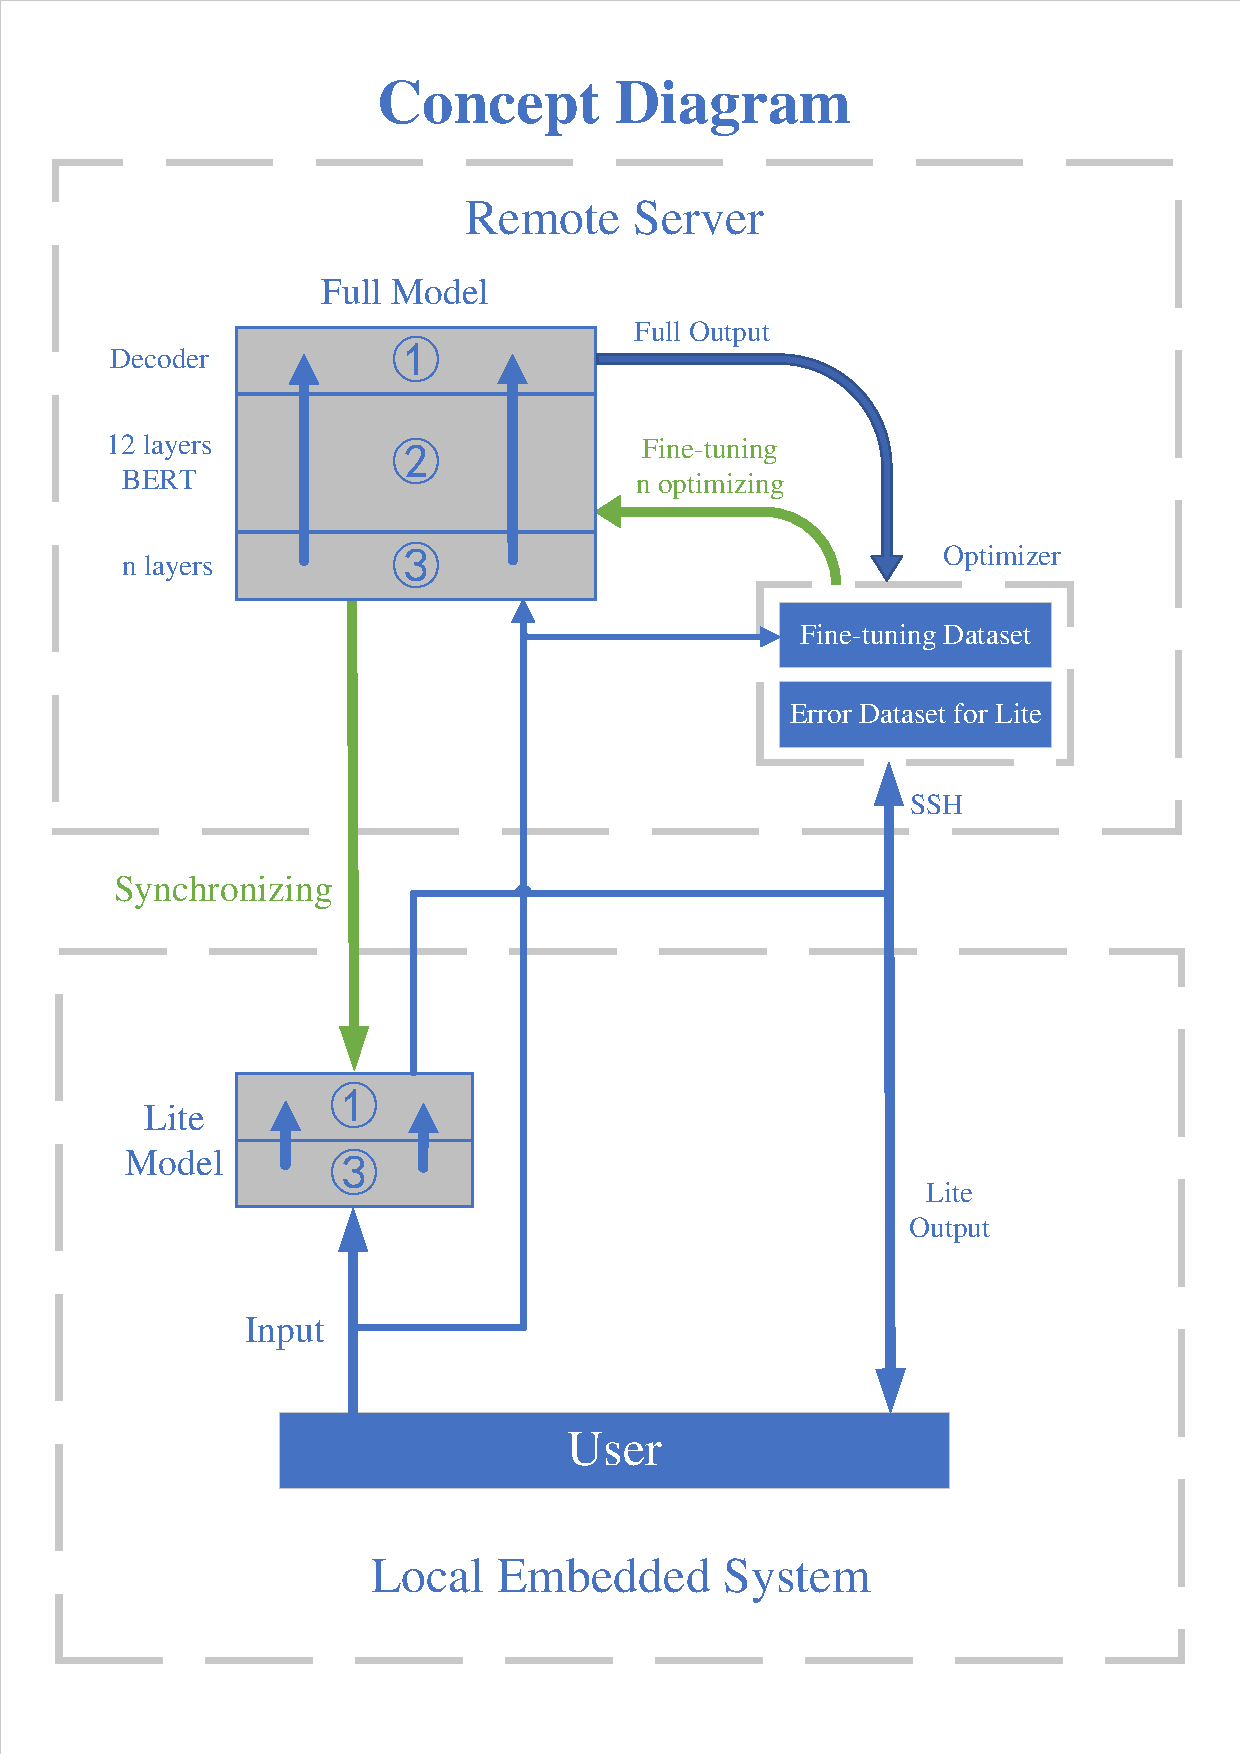
\includegraphics[width=0.45\textwidth]{Concept_Design.pdf}
    % \caption{Concept Design.}
\end{figure}
\end{frame}

\section{Shuocheng's Progress}

\section{Yihua's Progress}
\begin{frame}{\texttt{ALBERT} on Jetson TX2}
Try to run \texttt{ALBERT} with \texttt{tensorflow==1.15.2} on Jetson TX2.
\begin{block}{Difficulties}
AArch64 (ARMv8) platform is extremely poorly supported - no APT, no pip, even no wheels. Even Raspberry Pi (ARMv7) has better support. Most of the packages have to be compiled and built manually. Network was also a head-scratching problem.
\end{block}
\begin{itemize}
    \item Successfully installed JetPack 4.6 environment, which includes \texttt{CUDA==10.2}.
    \item Successfully built \texttt{bazel==0.26.1} with CUDA support.
    \item Successfully set up SSH/SFTP/SCP connections and proxies for AArch64 (ARMv8) platform.
    \item Failed to build \texttt{tensorflow==1.15.2} with \texttt{cuDNN==8.2.1} and \texttt{TensorRT==8.0.1-1+cuda10.2} because some incompatibilities are unresolvable.
\end{itemize}
\end{frame}
\begin{frame}{\texttt{ALBERT} on Jetson TX2}
\begin{block}{Difficulties}
Building \texttt{tensorflow} using \texttt{bazel} costs extremetly large disk space. It costs the remaining 31\% of the embedded disk \texttt{/dev/mmcblk0p1} or 2\% of the external disk (8.5 GiB), while \texttt{/dev/mmcblk0p1} only has 28768292 1K-blocks (28,094 MiB or 27.4 GiB). Beyond doubt it will cost disk space much more than this value.
\end{block}
When building caches occupy the whole disk space, Jetson TX2 system corrupted, which is dangerous. Referring to \url{https://blog.csdn.net/weixin_48695448/article/details/117337766}, it costs a lot of time to repair.
\begin{block}{Solution}
Use an external disk. Mount the disk, and specify the output path of \texttt{bazelbuild}.
\end{block}
\end{frame}
\begin{frame}{\texttt{ALBERT} on Jetson TX2}
All the experiences are summarized in \url{https://blog.csdn.net/yihuajack/article/details/121045347}. It might be easier to build a CPU-only version, but it is meaningless.
\begin{block}{Plan}
We have to use \texttt{TensorFlow 2} because migrating \texttt{ALBERT} from \texttt{tf1} to \texttt{tf2} is much more easier than migrating \texttt{tensorflow==1.15.2} from \texttt{cuDNN==7} to \texttt{cuDNN==8} and from \texttt{TensorRT==7} to \texttt{TensorRT==8}.
\end{block}
\begin{block}{Plan}
Accelerate the progress of building the application. The application takes speech audio as input, does speech recognition, converts speech to text, does NLP question-answering and computation offloading, and takes answers as output.
\end{block}
\end{frame}

\begin{frame}{\texttt{ALBERT} for TensorFlow 2}
Current solutions:
\begin{itemize}
    \item \href{https://github.com/kpe/bert-for-tf2}{bert-for-tf2}: 
    \item \href{https://github.com/kamalkraj/ALBERT-TF2.0}{ALBERT-TF2.0}: Lack of maintenance, last commit is on Dec 9, 2019.
    \item Issues of \href{https://github.com/google-research/albert}{ALBERT}.
\end{itemize}
Development approaches:
\begin{itemize}
    \item Start from ALBERT and put compability patches on it.
    \item Start from bert-to-tf2 and find possible ways to customize layers.
\end{itemize}
\end{frame}

\section{Albert}
\begin{frame}{Albert}
    \begin{block}{Preparation}
    \begin{enumerate}
        \item Configure the environment on the server
        \item Choose the pretrained model from \url{https://tfhub.dev/google/albert_large/3}
        \item Download the data set SQuAD from \url{https://rajpurkar.github.io/SQuAD-explorer/}
    \end{enumerate}
    \end{block}
\end{frame}

\begin{frame}[fragile]
\frametitle{Albert}
    \begin{block}{Result}
    \tiny
    \begin{lstlisting}
I0922 11:46:38.663871 140308634334976 run_squad_v2.py:505]
***** Final Eval results *****
INFO:tensorflow: exact = 50.09685841825992
I0922 11:46:38.663987 140308634334976 run_squad_v2.py:507] exact = 50.09685841825992
INFO:tensorflow: f1 = 50.11359538016659
I0922 11:46:38.664040 140308634334976 run_squad_v2.py:507] f1 = 50.11359538016659
INFO:tensorflow: null_score_diff_threshold = -1.230899453163147
I0922 11:46:38.664077 140308634334976 run_squad_v2.py:507]
null_score_diff_threshold = -1.230899453163147
INFO:tensorflow: total = 11873
I0922 11:46:38.664113 140308634334976 run_squad_v2.py:507] total = 11873
    \end{lstlisting}
    \end{block}
    The result is too low compared to the F1 score in the paper about 85.
\end{frame}

\begin{frame}{Albert}
    \begin{block}{Problems}
    \begin{enumerate}
        \item F1 score is too low compared to the F1 score in the paper
        \item The version of tensorflow is not consistent with the version in the embedded device
    \end{enumerate}
    \end{block}
    
    \begin{block}{Plans}
    \begin{enumerate}
        \item Solve the problems above
        \item Realize the function of updating the data set with the unsolvable questions from the lite model
    \end{enumerate}
    \end{block}
\end{frame}

\section{Early Exit}
\begin{frame}{Early Exit}
    \begin{figure}[H]
    \centering
    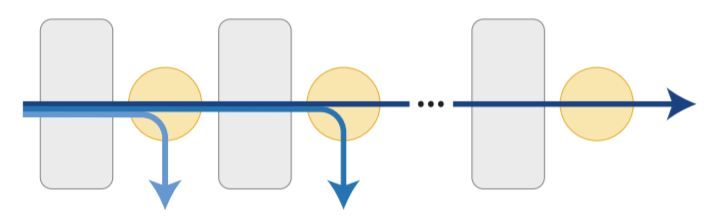
\includegraphics[width=0.6\textwidth]{early_exit.PNG}
    % \caption{Concept Design.}
    \end{figure}
    
    \begin{block}{}
    \begin{enumerate}[*]
        \item Grey blocks are transformer layers
        \item Orange circles are classification layers
        \item Blue arrows are possible exits
    \end{enumerate}
    \end{block}
\end{frame}

\begin{frame}{Early Exit}
    \begin{block}{Advantage}
    \begin{enumerate}[*]
        \item Prevent overfitting
        \item Reduce computation
    \end{enumerate}
    \end{block}
    
    \begin{block}{Characteristic}
    \begin{enumerate}[*]
        \item Match linguistically complex sentences with larger models and simple sentences with smaller models
        \item A lightweight classifier at the output of the transformer layer
        \item Threshold $E_T$
        \item Entropy
        \[H(x)=-\sum p(x)logp(x) = In(\sum^n_{k=1}e^{x_k})-\frac{\sum^n_{k=1}x_ke^{x_k}}{\sum^n_{k=1}x_k}\]
    \end{enumerate}
    \end{block}
\end{frame}

\begin{frame}{Early Exit}
    \begin{block}{Algorithm}
    for layer $i$ from 1 to $n$ do\\
    \qquad if $H(z_i) < E_T$ then \\
    \qquad \qquad return $z_i$\\
    \qquad end if\\
    end for\\
    if the question is solved \\
    \qquad return $z_n$\\
    else \\
    \qquad return unsolvable question to the server\\
    \end{block}
    \small{*$z_i$ is the output of each layer}
\end{frame}

\begin{frame}{Early Exit}
    \begin{block}{Plan}
    \begin{enumerate}[*]
        \item Realize the algorithm
        \item Apply the model to the data set SQuAD
        \item Test the different number of layers
    \end{enumerate}
    \end{block}
    

\end{frame}

\section{Future plan}
\begin{frame}{Future plan}
    \begin{columns}
	\column{0.5\textwidth}
	\begin{enumerate}[*]
        \item Synchronize the lite model with the full model
        \item Automatically update the data set on the server with the unsolvable questions on lite model 
        \item Migrate the model to the embedded device
    \end{enumerate}
	\bigskip
	\bigskip
	\bigskip
	\bigskip
	\bigskip
	\bigskip
	\column{0.5\textwidth}
	\begin{figure}[H]
    \centering
    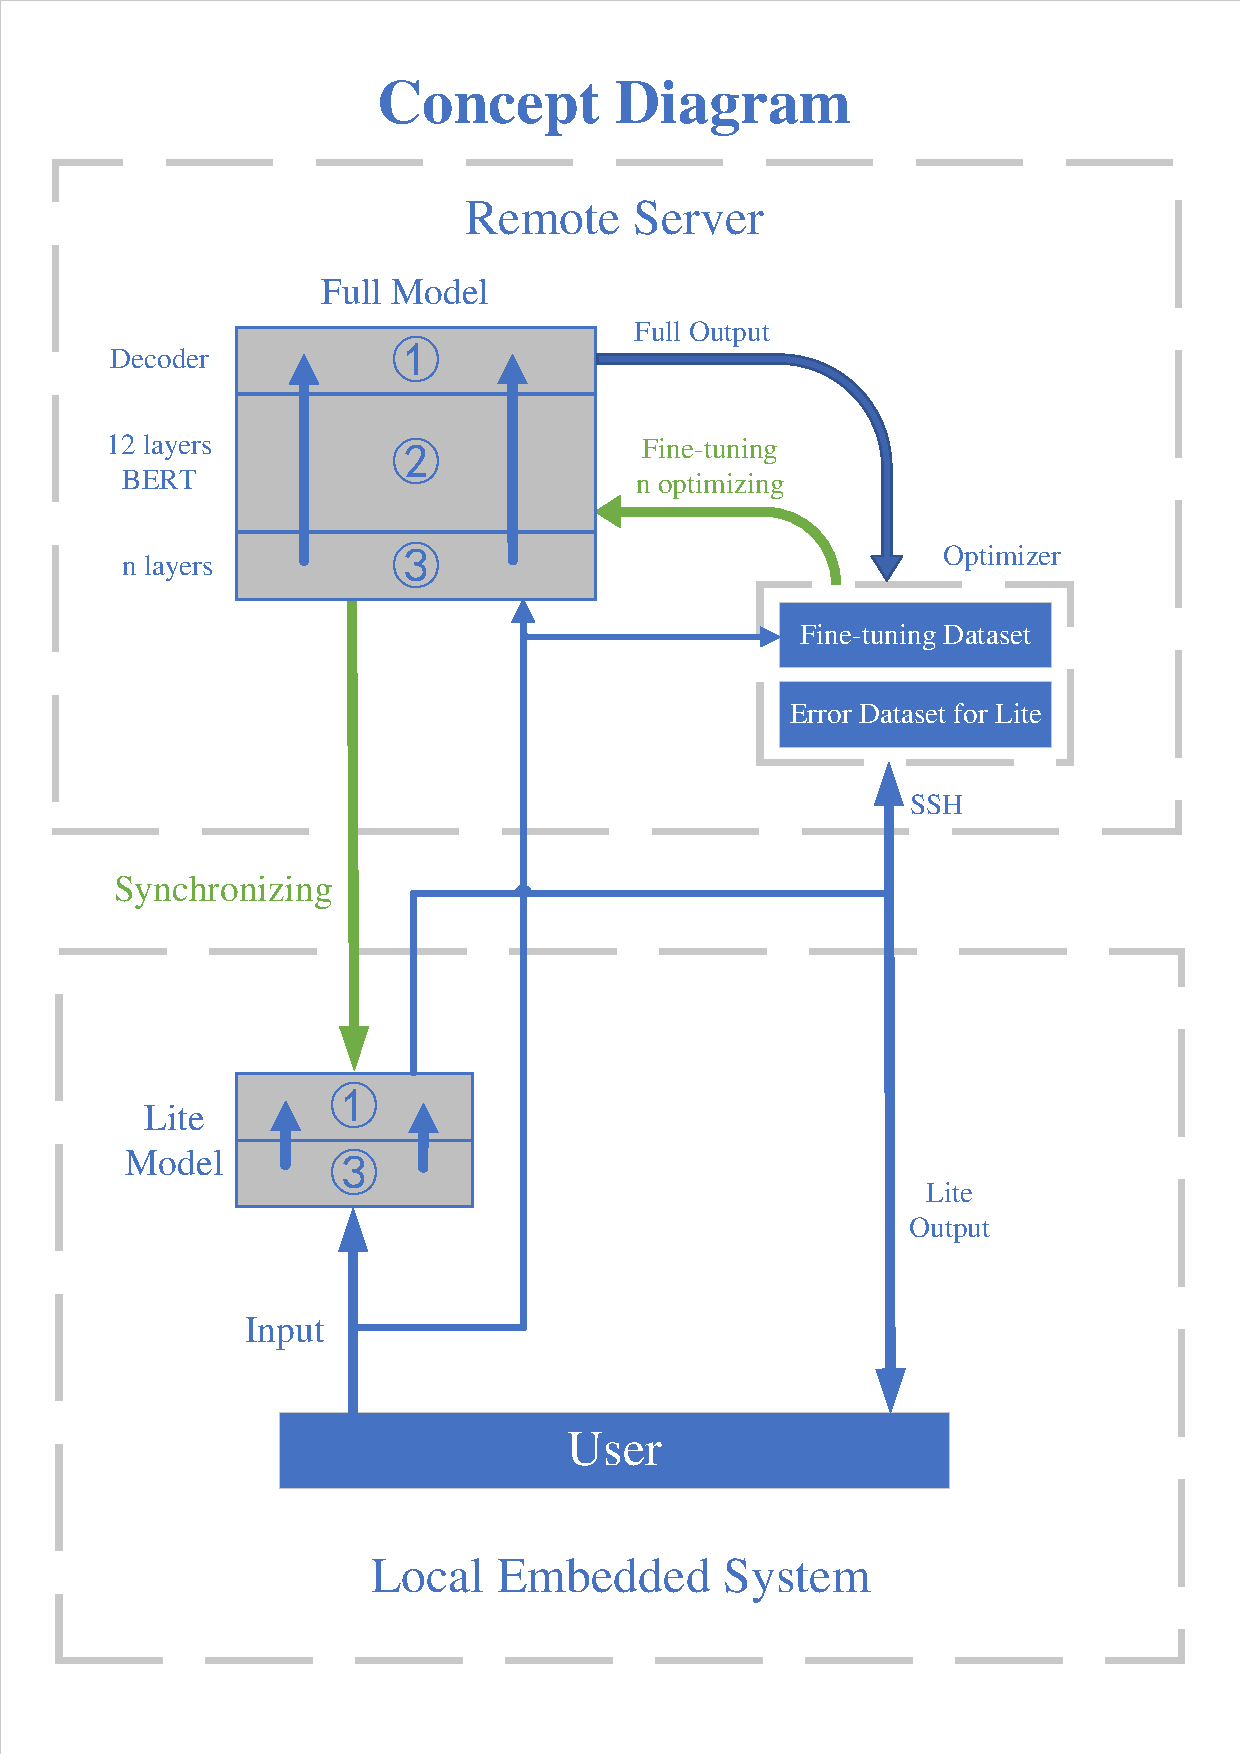
\includegraphics[width=0.9\textwidth]{Concept_Design.pdf}
    % \caption{Concept Design.}
    \end{figure}
\end{columns}
\end{frame}


%\section{Reference}
%\begin{frame}{Reference}
%    \printbibliography
%\end{frame}

\section{}
\begin{frame}{}
    \begin{center}
        \Huge Thanks!
    \end{center}
\end{frame}
\end{document}
